% ***************************************************************************************
% ************************************* CAPÍTULO I **************************************
% ***************************************************************************************
\chapter{MARCO TEÓRICO}
\thispagestyle{empty}

\abovedisplayskip=0pt
\belowdisplayskip=10pt
\abovedisplayshortskip=0pt
\belowdisplayshortskip=10pt

En este capítulo se exponen los fundamentos teóricos para el entendimiento del trabajo de diseño realizado. 

\section{Sistemas de control}
Un sistema de control está constituido por una cantidad de dispositivos mecánicos, eléctricos, electrónicos, que se organizan por diferentes niveles, pero que en conjunto utilizan un protocolo de comunicación determinado. Estos a su vez proporcionan la capacidad de gestionar y monitorizar diferentes procesos de acuerdo a su estructura utilizada. Históricamente, los sistemas de control se basan en dos capas, la capa de Control Digital Directo (DDC, \textit{Direct Digital Control}) por sus siglas en inglés y la capa de monitorización (SCADA  \textit{Supervisory control and data acquisition}) por sus siglas en inglés\cite{FundamentosControl}. Con los desarrollos tecnológicos y gracias a la interconexión con sistemas informatizados, se puede puede usar el término de BMS en gestión y supervisión de edificaciones, para definir indistintamente el sistema de control en su totalidad. Para empezar, se puede definir los diferentes niveles que componen un sistema BMS.

\begin{itemize}
    \item \textbf{Nivel de campo:} 
    este nivel se encarga de actuar o extraer información sobre los dispositivos utilizados en campo. Está compuesto por actuadores, sensores, módulos de E/S del sistema. Los módulos E/S se encargan de recoger las señales de los diferentes sensores y actuadores para incluirlas dentro del bus de comunicaciones del BMS.
    \item \textbf{Nivel de control:}
     está compuesto por la primera serie de controladores parametrizables y PLC(\textit{Programmable Logic Controller}). Estos se encargan de la recolección y procesado de datos, permiten también un preprocesamiento y lógicas locales autónomas de las instalaciones. En este nivel es importante garantizar el funcionamiento del sistema ante falla de comunicaciones con controladores de los niveles superiores. Por lo tanto si un controlador maestro falla o existen problemas en el bus de comunicación, el sistema puede seguir funcionando.
     \item \textbf{Nivel gestión:}
     este se compone por PC, servidores o PLC's. A este nivel los dispositivos se encargan de gestionar los distintos controladores utilizados en el nivel de control. Esta etapa es fundamental en términos de monitorización, ya que se recogen los datos de los niveles inferiores y con estos se generan los diferentes medios de presentación de información al usuario. También se le ofrece al usuario una interfaz interactiva con la cual el usuario pueda actuar con simplicidad según los datos visualizados.
     \item \textbf{Nivel usuario:}
     este nivel está compuesto por el conjunto de clientes que tienen acceso al nivel de control, pueden ser PC, móviles o clientes remotos. Los clientes cuentan con una interfaz especializada para conocer el estado total del sistema BMS, se puede configurar también esta interfaz según el tipo de usuario para permitir mayor o menor control sobre el sistema. 
\end{itemize}

\section{Elementos de un sistema BMS}

\subsection{Elementos de Campo}
\begin{itemize}
\item \textbf{Sensores:}
Es un objeto de capaz de detectar variables de instrumentación (magnitudes físicas o químicas), y a su vez transformarlas en variables eléctricas. A la hora de escoger cuál tipo de sensor utilizar se deben tener en cuenta las siguientes características:
\begin{itemize}
\item{Rango de medida:}
Dominio en el cual puede aplicarse el sensor.
\item{Sensibilidad:}
Mínima variación captada por el sensor.
\item{Precisión:}
Rango de error que puede ser presentado por el sensor.
\end{itemize}
\item \textbf{Actuadores:}
Son los dispositivos encargados de generar un efecto sobre un proceso con el fin de automatizarlo. Normalmente estos reciben una señal de un regulador o controlador, con lo cual generan una salida proporcional a la misma en el elemento final de control. Los actuadores se caracterizan por influir directamente en el proceso final de la automatización, esto con el fin de modificar la salida del proceso según las instrucciones obtenidas por la unidad de control. Para contemplar qué tipo de actuador es necesario seguir las mismas características contempladas para la escogencia de sensores.
\end{itemize}
\subsection{Elementos de Control}
\begin{itemize}
\item \textbf{Controlador Programable:}
Un controlador lógico programable, mejor conocido como PLC, es un dispositivo capaz de automatizar procesos electromecánicos, tales como el control de maquinarias, por ejemplo bombas de agua centrifugadas o control secuencial de relés. 

Un PLC se compone de una unidad de procesamiento central CPU e interfaces de entrada y salida, estas pueden ser de tipo analogicas o binarias. El procesador se encarga de ejecutar el programa escrito por el usuario, donde es posible la interacción de este con el exterior mediante sus puertos de comunicación. Mediante su interfaz de entrada es capaz de adaptar las señales provenientes de los elementos de entrada para que el CPU pueda interpretar dicha información. Además la interpretación de estas señales de entrada permiten una respuesta deseada por el usuario a través de las interfaces de salida que se encargan de activar algún elemento de campo. 

\item \textbf{Controlador Parametrizable:}
Un Controlador parametrizable se diferencia de un PLC, debido a que este no es libremente programable. Es decir, que se incluyen una programación previa sobre un problema en concreto; con la capacidad de ajustar ciertos parámetros sobre dicho problema. Un ejemplo sobre un controlador parametrizable es el de un controlador de
fancoil, el fabricante nos permitirá parametrizar las características básicas del fancoil para ajustar el controlador al sistema presente: 2 o 4 tubos, consignas, modos de funcionamiento, horarios, etc.

\item \textbf{Integraciones:}
Gracias a la existencia de un bus de comunicación, los distintos tipos de controladores tienen la capacidad de conectarse entre ellos, o con dispositivos de terceros. Mediante un mismo protocolo de comunicación, se puede compartir funciones, lógicas o parámetros entre los diferentes dispositivos conectados.

\end{itemize}

\subsection{Elementos de Gestión}
\begin{itemize}
\item \textbf{Software de Gestión:}
El sofware de gestión se encuentra por lo general en un PC o Servidor, con el cual se puede ejercer un control sobre la red BMS. Normalmente este software se dedica a la adquisición de datos obtenidos por los elementos de control.
\item \textbf{Web server:}
Un web server es la integración de la red BMS a una red con direcciones IP. Mediante su configuración correcta, esta ofrece la oportunidad de conectarse localmente o de forma remota al sistema BMS.
\item \textbf{Software Gráfico:}
Este se encarga de brindar al usuario la capacidad de visualizar el sistema mediante paneles o gráficos. Por lo general se puede incluir pantallas o paneles realizados mediante este software gráfico al web server, para la visualización de usuarios no operarios.
\end{itemize}
\subsection{Elementos de Usuarios}
\begin{itemize}
\item \textbf{PC de usuario:}
PC convencional capaz de acceder mediante un navegador web al web server para supervisión y control del sistema BMS de una manera cómoda y sencilla. Mediante una correcta configuración se puede adaptar esta para diferentes tipos de usuarios, según las funciones que desempeñe y sus conocimientos.
\item \textbf{Dispositivos móviles:}
Teléfonos celulares o tablets, que mediante su navegador en el caso que dispongan o APP's pueden realizar el acceso al web server y tener visualización del sistema.

\end{itemize}

\section{Protocolo BACnet MS/TP}

Este protocolo diseñado originalmente por la \textit{American Society of Heating, Refrigerating and Air-Conditioning Engineers} ASHRAE, actualmente es un estándar de la ISO 16484-5 y ANSI 135\cite{BACnetProtocol}, que asegura la compatibilidad e intercambiabilidad entre equipos de diferentes fabricantes.

\subsection{Estructura del sistema:}
El protocolo BACnet MS/TP es un protocolo bidireccional con una estructura de múltiple maestros-esclavos basado en el paso de tokens. Solo los dispositivos maestros pueden recibir el token, y solo el dispositivo que lo tiene puede originar un mensaje en el bus. El token pasa entre dispositivos maestros a través de un pequeño mensaje, este se pasa en orden consecutivo comenzando con la dirección más baja entre el grupo de direcciones del bus. Los dispositivos esclavos solo se comunican en el bus cuando respondes a solicitudes de datos desde un dispositivo maestro. 

Normalmente se utiliza un bus MS / TP para dos tipos de buses: un bus de controlador de campo (FC, \textit{Field Controller}) y un bus actuador de sensor (SA, \textit{Sensor Actuator}). En la Figura \ref{fig:BACnet_MSTP} podemos observar un ejemplo de implementación de un bus BACnet MS/TP.

\begin{figure}[H]
    \centering
    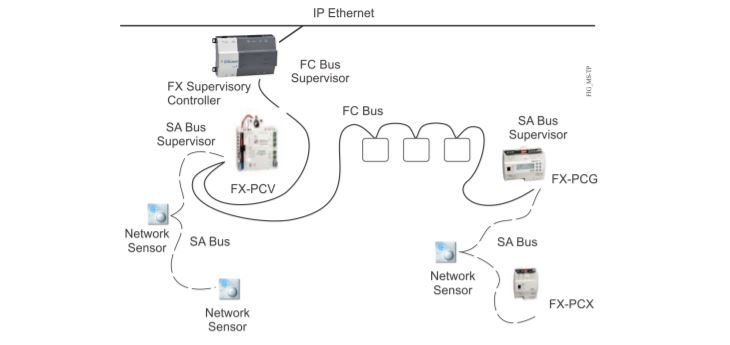
\includegraphics[width=1\textwidth]{2_MainMatter/Capitulo1/Imagenes/BACnet_MSTP_Johnson.JPG}
    \caption{Ejemplo de un bus de comunicaciones MS/TP\cite{MSTP}}
    \label{fig:BACnet_MSTP}
\end{figure}

El bus FC y el bus SA son redes de dispositivos conectados en cadena. Cada bus tiene solo un bus supervisor, dependiendo de qué controladores están conectados. En un bus local de FC, el supervisor de este es el controlador supervisor. En el bus SA local, el supervisor del bus es un controlador de campo.

El supervisor del bus se comunica con los dispositivos del bus supervisado y con los dispositivos del siguiente (nivel superior) bus en la red. El supervisor del bus FC generalmente inicia la comunicación en el FC bus o SA bus.

\section{Protocolo N2}
El bus de comunicación N2, es un protocolo desarrollado por Johnson Controls de red local que une controladores e interfaces al módulo de control de red(NCM \textit{network control module}). Este protocolo fue desarrollado principalmente para conectar los controladores desarrollados por Johnson Controls con sus dispositivos de campo.

\subsection{Estructura del sistema:}
El bus N2 utiliza un protocolo maestro/esclavo, en el cual es dispositivo maestro (NCM), inicia la comunicación con los dispositivos del bus N2. El bus N2 está conectado en cadena, en el que múltiples dispositivos están conectados en serie. A diferencia del protocolo BACnet, el bus N2 se comunica sólo entre el dispositivo maestro (NCM) y los dispositivos conectados en el mismo lazo. Sin embargo, para comunicarse entre dispositivos de más alto nivel, se utiliza el bus tipo N1 u otro protocolo de comunicación. Podemos observar un ejemplo de implementación de este bus en la Figura \ref{fig:N2}

\begin{figure}[H]
    \centering
    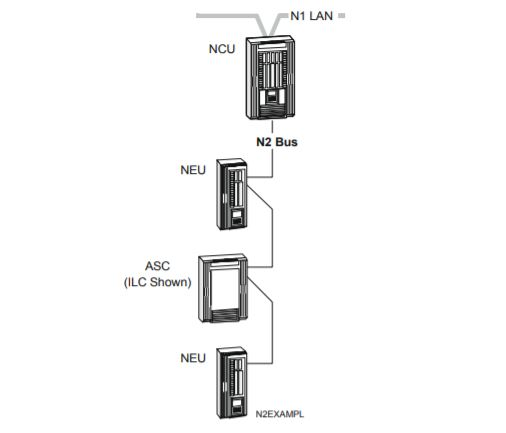
\includegraphics[width=0.60\textwidth]{2_MainMatter/Capitulo1/Imagenes/N2_Johnson.JPG}
    \caption{Ejemplo de un bus de comunicaciones N2\cite{N2}}
    \label{fig:N2}
\end{figure}